%********BEGIN PREAMBULE*********
\documentclass[14pt,a4paper]{report}

\usepackage[14pt]{extsizes}
\usepackage{cmap}
\usepackage[T2A]{fontenc}
\usepackage[utf8]{inputenc}
\usepackage[english,russian]{babel}
\usepackage{pscyr}

\usepackage{graphicx}
\usepackage{amssymb,amsfonts,amsmath,amsthm}
\usepackage{lscape}
\usepackage{makecell}
\usepackage{multirow}
\usepackage{ulem}
\usepackage{indentfirst}
\usepackage{setspace}
\usepackage{color}
\usepackage{tabularx}
\usepackage{titlesec}
\usepackage{hyperref}
\hypersetup{pdfborder = 0 0 0}
\usepackage{tocloft}
\usepackage{listings}
\usepackage{float}

% Ключевые слова
\newcommand{\kwTitle}{Разработка системы для создания и редактирования документов на языке LaTeX}
\newcommand{\kwPlace}{Томск}
\newcommand{\kwYear}{2014}
\newcommand{\kwAuthorName}{Ветров А.А.}
\newcommand{\kwAuthorFaculty}{Кибернетики}
\newcommand{\kwAuthorSpeciality}{Информационные системы и технологии}
\newcommand{\kwAuthorDepartment}{Вычислительной техники}
\newcommand{\kwAuthorInfo}{студент гр. 8И32}
\newcommand{\kwTeacherName}{Хаустов П.А.}
\newcommand{\kwTeacherTitle}{Руководитель}
\newcommand{\kwTeacherInfo}{Ассистент кафедры ВТ}

\lstset{
	language=C++,                % choose the language of the code
	basicstyle=\footnotesize\ttfamily,       % the size of the fonts that are 
	%used for 
	%the code
	numbers=left,                   % where to put the line-numbers
	numberstyle=\footnotesize,      % the size of the fonts that are used for 
	%the line-numbers
	stepnumber=1,                   % the step between two line-numbers. If it 
	%is 1 each line will be numbered
	numbersep=5pt,                  % how far the line-numbers are from the 
	%code
	backgroundcolor=\color{white},  % choose the background color. You must 
	%add \usepackage{color}
	showspaces=false,               % show spaces adding particular underscores
	showstringspaces=false,         % underline spaces within strings
	showtabs=false,                 % show tabs within strings adding 
	%particular underscores
	%frame=single,           % adds a frame around the code
	tabsize=2,          % sets default tabsize to 2 spaces
	captionpos=b,           % sets the caption-position to bottom
	breaklines=true,        % sets automatic line breaking
	breakatwhitespace=false,    % sets if automatic breaks should only happen 
	%at whitespace
	escapeinside={\%*}{*)},          % if you want to add a comment within 
	%your code
	%keywordstyle=\color{blue},
	%stringstyle=\color{red},
	%commentstyle=\color{green}
}

\usepackage[tableposition=top]{caption}
\usepackage{subcaption}
\DeclareCaptionLabelFormat{gostfigure}{Рисунок #2}
\DeclareCaptionLabelFormat{gosttable}{Таблица #2}
\DeclareCaptionLabelSeparator{gost}{~---~}
\captionsetup{labelsep=gost}
\captionsetup[figure]{labelformat=gostfigure}
\captionsetup[table]{labelformat=gosttable}
\renewcommand{\thefigure}{\arabic{figure}}
\renewcommand{\thesubfigure}{\asbuk{subfigure}}

\onehalfspacing % полуторный интервал
\renewcommand{\rmdefault}{ftm} % Times New Roman
\frenchspacing % не всталять дополнительный пробел в конце предложения
%\spaceskip .45em plus .4em minus .0em

\usepackage{geometry} % поля
\geometry{left=3cm}
\geometry{right=1cm}
\geometry{top=2cm}
\geometry{bottom=2cm}

\usepackage{fancyhdr} % колонитулы
\pagestyle{fancy}
\fancyhf{}
\fancyfoot[R]{\thepage}
\fancyheadoffset{0mm}
\fancyfootoffset{0mm}
%\setlength{\headheight}{17pt}
%\setlength{\footheight}{17pt}
\renewcommand{\headrulewidth}{0pt}
\renewcommand{\footrulewidth}{0pt}
\fancypagestyle{plain}
{
    \fancyhf{}
    \fancyfoot[R]{\thepage}
}

% Заголовки

\titleformat{\chapter}
    {\bfseries}
    {\thechapter.}
    {1em}{}
 
\titleformat{\section}
    {\normalsize\bfseries}
    {\thesection}
    {1em}{}
 
\titleformat{\subsection}
    {\normalsize\bfseries}
    {\thesubsection}
    {1em}{}

% Оглавление

\newcommand{\prechapterheading}[1]{
	\clearpage 
    \begin{center}
    \textbf{#1}
    \end{center}
}

\makeatletter
\newif\if@prechapterused
\@prechapterusedfalse

\newcommand{\l@prechapter}[2]{#1\cftdotfill{\cftdotsep}#2\par}
\newcommand{\prechapter}[1]{
	%\chapter{#1}    
    \prechapterheading{#1}
    \@prechapterusedtrue
    \addcontentsline{toc}{chapter}{#1}
}

\let\oldchapter\chapter

\renewcommand{\chapter}[1]
{
\if@prechapterused\vspace{-2em}\@prechapterusedfalse\fi
\begingroup
	\let\clearpage\relax
	\let\cleardoublepage\relax
	\oldchapter{#1}
\endgroup
}
\makeatother

\renewcommand{\cfttoctitlefont}{\hspace{0.38\textwidth} \bfseries}
\renewcommand{\cftbeforetoctitleskip}{-1em}
\renewcommand{\cftaftertoctitle}{\mbox{}\hfill \\ \mbox{}\hfill{\footnotesize Стр.}\vspace{-2.5em}}
\renewcommand{\cftchapfont}{\normalfont}
\renewcommand{\cftchapdotsep}{\cftdotsep}
\renewcommand{\cftchapleader}{\normalfont\cftdotfill{\cftchapdotsep}}
\renewcommand{\cftchappagefont}{\normalfont}
\renewcommand{\cftsecfont}{\hspace{31pt}}
\renewcommand{\cftsubsecfont}{\hspace{11pt}}
\renewcommand{\cftbeforechapskip}{1em}
\renewcommand{\cftbeforesecskip}{1em}
\renewcommand{\cftsecindent}{-0.5em}
\renewcommand{\cftparskip}{-2mm}
\renewcommand{\cftdotsep}{1}
\setcounter{tocdepth}{1} % задать глубину оглавления — до section включительно

% Настройка вертикальных и горизонтальных отступов в заголовках
\titlespacing*{\chapter}{\parindent}{*4}{*0}
\titlespacing*{\section}{\parindent}{*4}{*4}
\titlespacing*{\subsection}{\parindent}{*0}{*0}

\setlength{\parindent}{15mm} % абзацный отступ

\usepackage{enumitem}
\setlist{noitemsep}
\setlist[enumerate]{leftmargin=4em}
\setlist[itemize]{leftmargin=4em}

\newcommand{\handtextplace}[2][50px]
{
	\parbox{#1}{
	\begin{center}
		{~}\\[-0.005\textheight]
		\underline{\hspace{#1}}
		\\[-0.005\textheight]\footnotesize{#2}
	\end{center}
	}
}

\newcommand{\textplace}[2]
{
	\parbox{\textwidth}{
	\begin{center}
		{~}\\[-0.005\textheight]
		#1
		\\[-0.005\textheight]\footnotesize{(#2)}
	\end{center}
	}
}

\begin{document}

\thispagestyle{empty}

\begin{small}

\begin{center}
\textbf{Министерство образования и науки Российской Федерации}\\
Федеральное государственное автономное образовательное учреждение высшего образования\\
\textbf{<<НАЦИОНАЛЬНЫЙ ИССЛЕДОВАТЕЛЬСКИЙ\\ТОМСКИЙ ПОЛИТЕХНИЧЕСКИЙ 
УНИВЕРСИТЕТ>>}\\
\end{center}
\hrule

\begin{flushleft}
Институт \hspace{2em} \kwAuthorFaculty\\
Направление подготовки (специальность) \hspace{2em} \kwAuthorSpeciality\\
Кафедра \hspace{2em} \kwAuthorDepartment\\
\end{flushleft}

\vspace{5pt}

\begin{center}
\textbf{ПОЯСНИТЕЛЬНАЯ ЗАПИСКА}\\
\textbf{к творческому проекту}\\
\end{center}
на тему <<\kwTitle>>

\noindent\begin{tabularx}{\textwidth}{Xrr}
\raggedright{Выполнил} \kwAuthorInfo & \handtextplace[100pt]{(подпись)} & 
\kwAuthorName\\*[-30pt]
~ & ~ &
\handtextplace[30pt]{~}~\handtextplace[100pt]{(дата 
сдачи)}~20\handtextplace[20pt]{~}г.\\*[10pt]
\kwTeacherTitle & \kwTeacherInfo & 
\kwTeacherName\\*[0pt]
~ & \handtextplace[100pt]{(оценка руководителя)} & 
\handtextplace[100pt]{(подпись)}\\*[-20pt]
~ & ~ & 
\handtextplace[30pt]{~}~\handtextplace[100pt]{(дата 
проверки)}~20\handtextplace[20pt]{~}г.\\*[10pt]
Творческий проект & студент \kwAuthorName & выполнил и защитил\\*[0pt]
~ & ~ & с оценкой \handtextplace[100pt]{~}\\*[-30pt]
Члены комиссии: & \handtextplace[100pt]{~} & ~\\*[-30pt]
~ & \handtextplace[100pt]{~} & ~\\*[-30pt]
~ & \handtextplace[100pt]{~} & ~\\*[-30pt]
~ & ~ & 
\handtextplace[30pt]{~}~\handtextplace[100pt]{(дата 
защиты)}~20\handtextplace[20pt]{~}г.\\*[10pt]
\end{tabularx}

\vspace{30mm}

\noindent{
\kwPlace~\kwYear~г.
}

\end{small}

\newpage

\vspace*{-3em}

\chapter{Задание}
В рамках проектной деятельности студенту необходимо создать программное 
обеспечение для создания и редактирования документов на языке разметки LaTeX через веб-интерфейс.
Данный продукт должен позволять пользователю абстрагироваться от самого языка и редактировать документы
путем взаимодействия с интерактивными элементами, расположенными на web-странице. В конце концов пользователь
должен получить документ на языке разметки LaTeX, который после компиляции должен давать документ, оформленный
по стандартам учебного учреждения.

\chapter{Реферат}
Для создания документации и редактирования документов на языке разметки LaTeX было разработанно web-приложение, написанное на языке программирования JavaScript с использованием фреймворка AngularJS и оформленное с помощью Twitter Bootstrap. В ходе разработки были спроектированы и написаны интерфейс пользователя, обработчик LaTeX шаблона и компоненты внутреннего устройства, необходимые для работы программы. Приложение было протестировано, с помощью него был написан отчет по дисциплине <<Программирование на ЯВУ>>. Данное приложение размещается в сети интернет.

\newpage

\tableofcontents
\newpage

\vspace*{-12pt}
\chapter{Определения}
\textbf{LaTeX} --- система компьютерной верстки, предназначенная для описания содержания и структуры документа,
а также формирующая на основе выбранного шаблона оформленный и готовый для распечатки документ.

\textbf{HTML5 (HyperText Markup Language, version 5)} --- язык для 
структурирования и 
представления содержимого всемирной паутины.

\textbf{CSS3 (Cascading Style Sheets 3)} --- формальный язык разметки, 
используемый как 
средство описания и оформления внешнего вида веб-страниц

\textbf{JavaScript} --- прототипно-ориентированный сценарный язык 
программирования, 
встраиваемый в браузер для программного доступа к объектам приложений

\textbf{MVC} --- принцип разработки приложений, согласно которому оно должно иметь модель, представление и контролер, взаимодействующие друг с другом.

\chapter{Обозначения и сокращения}

\textbf{ТПУ} --- Национальный исследовательский Томский политехнический университет

\chapter{Введение}

Многим студентам в ходе обучения приходится писать множество разнообразных документов, таких как
отчеты по лабораторным работам, рефераты, курсовые и дипломные работы и так далее, причем каждый документ
должен быть оформлен по стандартам ТПУ. В итоге на оформление отчетности может уйти больше времени, чем на саму работу.
Для облегчения жизни студентов было решено создать такую систему, которая позволит упростить создание документации. Также данная система должна хранить в себе стандартные шаблоны оформления работ, чтобы уменьшить время на создание структуры документа.
Полученная система не должна зависеть от программного обеспечения, установленного на компьютере, поэтому она должна быть доступна через интернет.

\newpage
\chapter{Цель проекта}

Получить навыки работы с издательской системой LaTeX, а также с технологиями создания современных web-приложений на основе технологий HTML5 и JavaScript.

\chapter{Задачи проекта}

\begin{itemize}
\item Разработка концепции проекта, рабочего плана и плана развития проекта;
\item Проектирование внутренней части системы;
\item Проектирование интерфейса пользователя;
\item Написание программного кода;
\item Тестирование реализованного функционала.
\end{itemize}

\chapter{Основная часть работы}
Начальный этап работы состоял в том, чтобы выбрать технологии, на которых будет разрабатываться приложение. Так как приложение должно работать в web-браузере, был выбран язык программирования JavaScript, который является наиболее распространенным скриптовым языком программирования. Для него был выбран MVC фреймворк AngularJS, который формирует структуру приложения, а также библиотеки Twitter Bootstrap, предназначенные для оформления внешнего вида.

После этого были спроектирована структура приложения. Согласно парадигме MVC в приложении необходимы модель, представление и контролер. В качестве модели выступает сервис DocumentService, обеспечивающий хранение и обработку информации, содержащейся в документе, а также сервис NavigationSerivce, хранящий структуру документа для перемещения по ней. В качестве представления были созданы директивы Tree, отображающая дерево документа и Paragraph, отображающая блоки текста в документе. В качестве контроллера был создан модель Editor, связывающий все компоненты вместе.

\begin{figure}[H]
\centerline{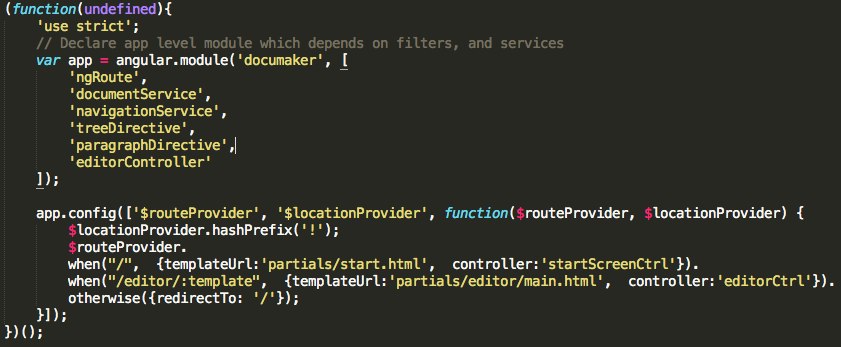
\includegraphics[scale=0.4]{gfx/1.png}}
\caption{Конфигурации компонентов AngularJS}
\label{fig1}
\end{figure}

После этого был спроектирован интерфейс пользователя. Для этого были созданы HTML шаблоны для каждого интерактивного элемента, присутствующего в редакторе, которые отображаются соответствующими директивами. В шаблонах используются элементы Twitter Bootstrap, которые позволяют оформить компоненты ровно и красиво.

\begin{figure}[H]
\centerline{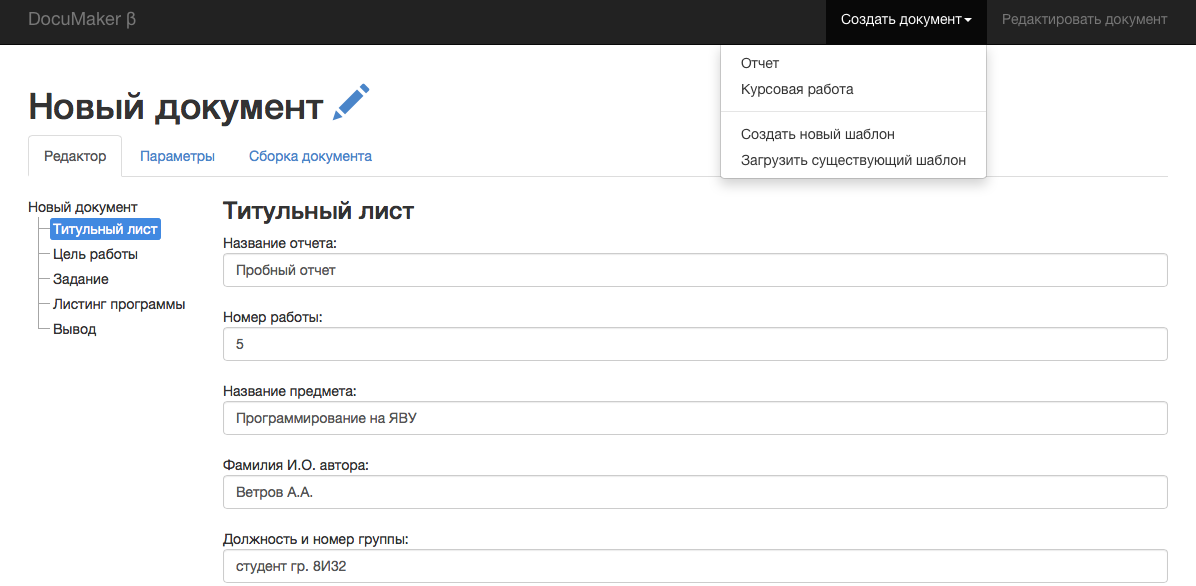
\includegraphics[scale=0.4]{gfx/2.png}}
\caption{Оформление редактора}
\label{fig2}
\end{figure}

После этапа проектирования был написан код, реализующий web-
приложение согласно проекту. Для проверки работы программы был написан отчет по дисциплине <<Программирование на ЯВУ>>. Отчет, сформированный программой соответствовал ожиданиям.
\begin{figure}[H]
\centerline{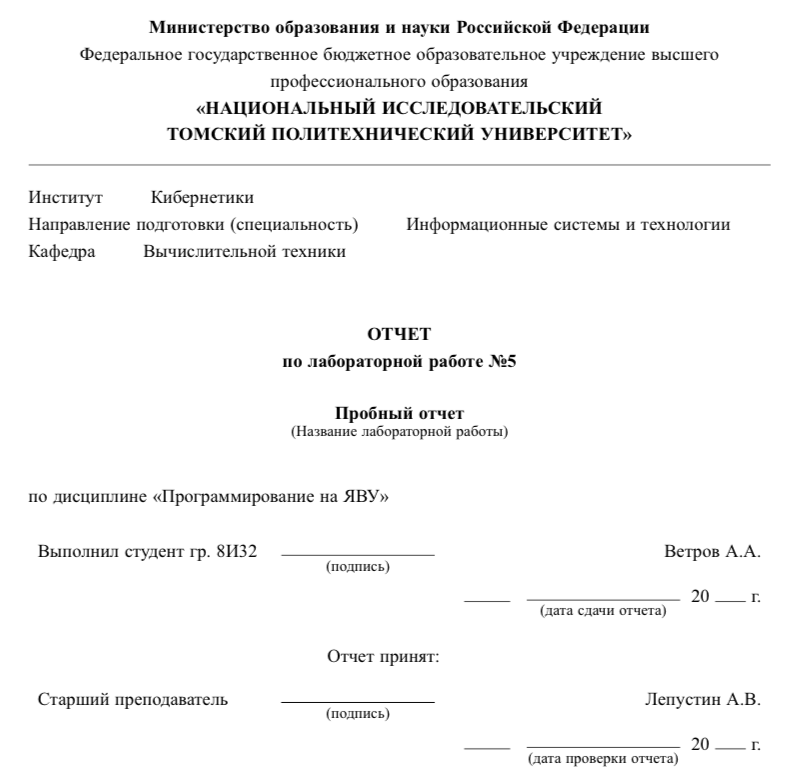
\includegraphics[scale=0.4]{gfx/3.png}}
\caption{Тестовый отчет}
\label{fig3}
\end{figure}

\chapter{Результаты выполнения работы}

В ходе проделанной работы был разработан программный продукт в виде Web-приложения для 
создания и редактирования документов на языке разметки LaTeX. Данный 
продукт был выполнен с помощью современных средств разработки Web-приложений, 
таких как HTML5, CSS3 и JavaScript. На данном этапе удобство пользования данным продуктом не было приоритетной задачей, но
в дальнейшем планируется развитие продукта до конечного состояния, при котором его можно использовать в коммерческих целях.

\chapter{Список использованных интернет-ресурсов}

\begin{enumerate}
  \item htmlbook.ru [Электронный ресурс] // Режим доступа: http://htmlbook.ru.
  \item ECMAScript 5 на русском [Электронный ресурс] // Режим доступа: http://es5.javascript.ru.
  \item LaTeX -- A document preparation system [Электронный ресурс] // Режим доступа: http://www.latex-project.org.
\end{enumerate}

\chapter{Перечень использованных программных продуктов}

\begin{enumerate}
  \item \textbf{SublimeText} --- быстрый кроссплатформенный редактор исходных 
  текстов программ.
  \item \textbf{NodeJS} --- веб-сервер.
  \item \textbf{Twitter Bootstrap} --- свободный набор инструментов для создания сайтов и веб-приложений.
  \item \textbf{AngularJS} ---  JavaScript-фреймворк с открытым исходным кодом, предназначен для разработки одностраничных приложений.
\end{enumerate}
\end{document}